\documentclass[final]{beamer}
\usetheme{RJH}
\usepackage[orientation=portrait,size=a1,scale=1.4,debug]{beamerposter}
\usepackage[absolute,overlay]{textpos}
\usepackage{amsmath,amsfonts,amssymb}
\usepackage{color}
\setlength{\TPHorizModule}{1cm}
\setlength{\TPVertModule}{1cm}

%
\includegraphics[height=2cm,width=3cm]{ANU_LOGO_cmyk_56mm.pdf}
\title{Open Software - Restricted Data: The Suicide/Climate Case}
\author{Ivan Hanigan$^1$, David Fisher$^2$, Steven McEachern$^3$}
\footer{More information from \texttt{ivan.hanigan@gmail.com} or at \texttt{http://opensoftware-restricteddata.github.io}}
\date{}

\begin{document}

%\begin{textblock}{6}(0.,0.2)
%
\includegraphics[width=3cm]{ANU_LOGO_cmyk_56mm.png}
%\end{textblock}

\begin{frame}{} 

\begin{textblock}{17}(2,5)
\begin{block}{Restricted Data is Safe}
\begin{scriptsize}
Restrictions on access to confidential health data have increased recently. Enabling safe access to data and analytic software is needed to address the {\color{red}\textbf{Replicability Crisis}} (Peng 2011).  We present an environment for analysing restricted data using open software. The system is described in Figure~\ref{fig:sys} and a Case Study of the historical association of suicides with climate (and extrapolation of this under climate change/adaptation scenarios) in the bottom half of the poster. These tools allow users to access restricted data; protects confidentiality and allows use of open software for reproducibility (King~1995).  
\end{scriptsize}
\end{block}

\begin{block}{Restrictive IT Environments}
\begin{scriptsize}
Previous solutions to this challenge make access so restricted that usability is compromised. We aimed to build a collection of tools for the conduct of many types of health and social science research. The starting point for users is the data catalogue, which provides for finding data available from the store of {\color{red} Restricted data} and {\color{blue}Less~Restricted data}  for approved use. Once data are discovered, the researcher has capacity to manipulate the datasets on the secure server. The PostgreSQL database integrates and Geoserver visualises, while statistical tools are available in the R-studio server browser.
\end{scriptsize}  

\end{block}
\end{textblock}

\begin{textblock}{17}(21.25,5)
\begin{block}{Server-Client Architecture}
\begin{figure}[!h]
\centering
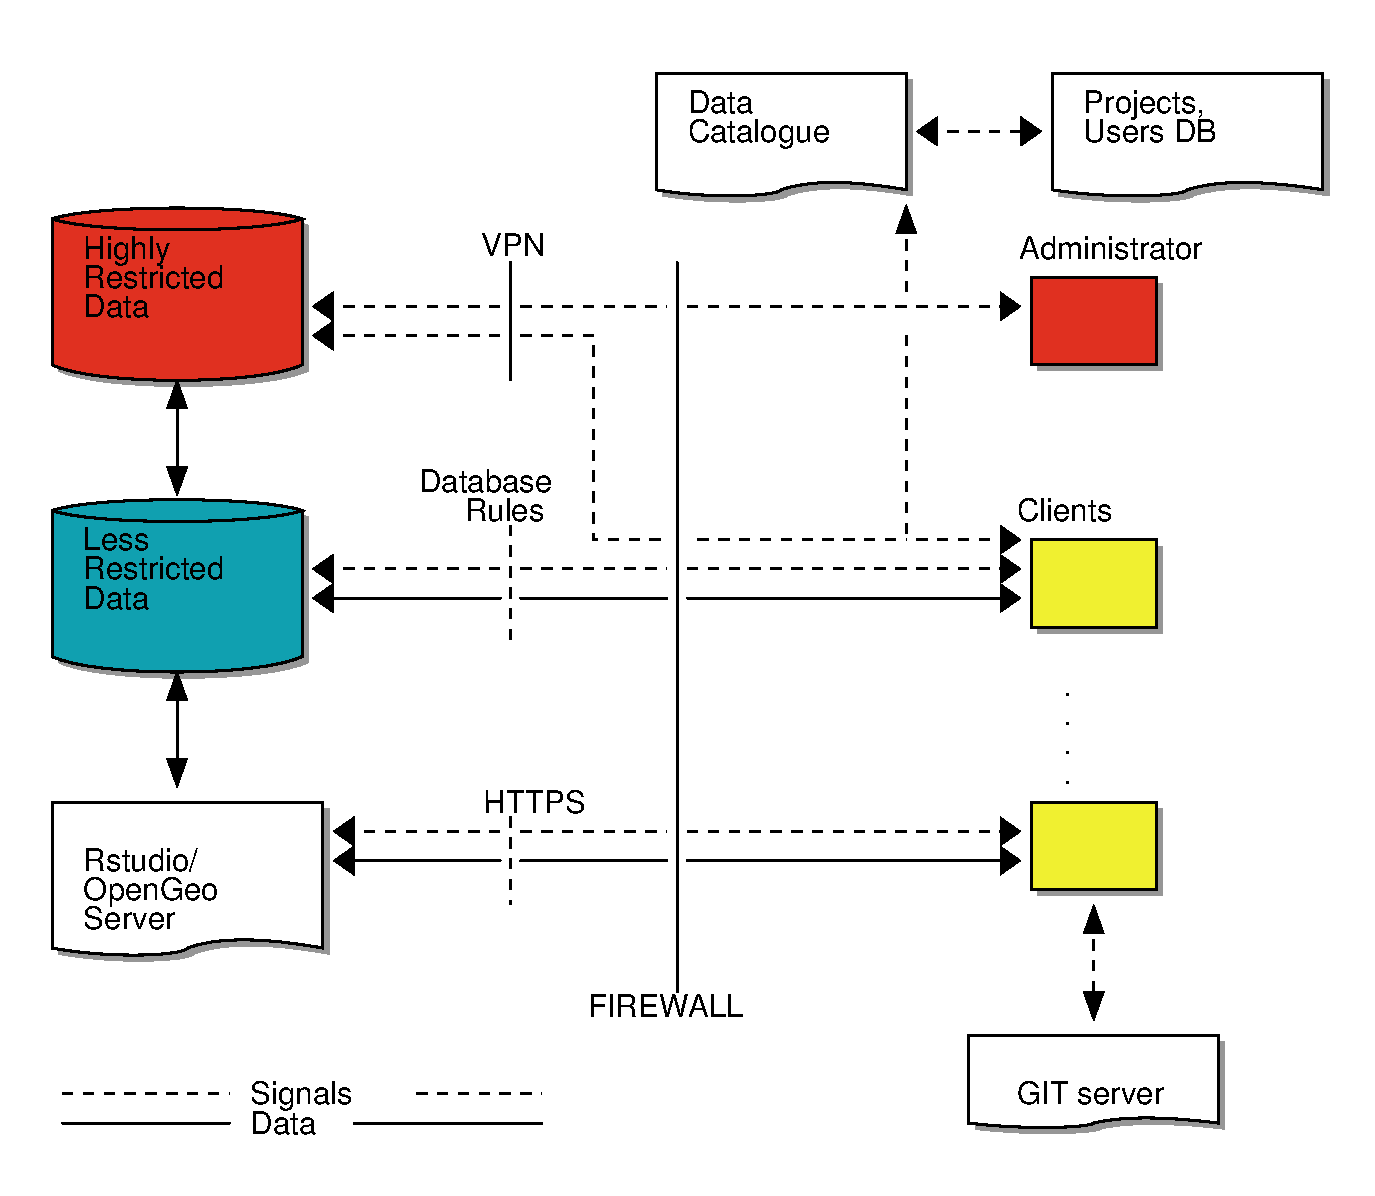
\includegraphics[width=\textwidth]{opensoft.pdf}
\caption{1. System Design}
\label{fig:sys}
\end{figure}
\end{block}

\begin{block}{The Stack}
\begin{tiny}
\textbf{Hardware}:
\begin{itemize}
\item National Research Cloud \emph{http://www.nectar.org.au/research-cloud/}
\item Centos 6.4 \emph{www.centos.org/}
\end{itemize} 

\textbf{Database (The Brawn)}:
\begin{itemize}
\item PostgreSQL 9.2 \emph{http://www.postgresql.org/}
\item PostGIS 2.0 \emph{http://postgis.refractions.net/}
\end{itemize} 

\textbf{Analysis (The Brains)}:
\begin{itemize}
\item R language for statistical computing \emph{http://www.r-project.org/}
\item Rstudio server \emph{www.rstudio.com/‎}
\item OpenGeo Suite \emph{http://opengeo.org/}
\end{itemize} 

\textbf{Information Management:}
\begin{itemize}
\item Projects,UsersDB Oracle XE APEX \emph{www.oracle.com}
\item Data Catalogue \emph{http://assda.anu.edu.au/ddiindex.html}
\end{itemize}

\textbf{The Client Side}:
\begin{itemize}
\item The Kepler Project \emph{https://kepler-project.org/‎}
\item pgAdmin \emph{www.pgadmin.org/‎}
\item Git Version Control and GitHub \emph{https://github.com/}
\end{itemize}


\end{tiny}
\end{block}

\end{textblock}

\begin{textblock}{17}(40.5,5)

\begin{block}{Reproducibility}
\begin{scriptsize}
Such analytical tools will enhance the ability of adaptive management practitioners to assess the potential influence of adaptations. The use of the system shows the ease with which multiple data sources (some restricted) can be analysed in a secure way using open software. This will build capacity to answer complex research questions and compare multiple climate change scenarios or adaptation assumptions; achieving simultaneous vision of potential future outcomes from different standpoints.
\end{scriptsize}  

\end{block}

\begin{block}{How it works}
\begin{scriptsize}
\begin{itemize}
\item Open a web browser / log on to the catalogue / find data
\item In the web browser log on to Rstudio server
\item Connect to database / query datasets / join / subset / transform
\item Get data to your Rstudio server workspace and analyse
\item Commit all code to GitHub, download resulting dataset and reports 
\end{itemize}
\end{scriptsize}
\end{block}

\begin{block}{Summary}
\begin{scriptsize}
This system:
\begin{itemize}
\item Assists rigorous data management practices
\item Enables multiple data sources (some restricted) to be analysed
\item Storage of data is secure
\item Analytic code is made available as open software
\end{itemize}


\begin{itemize}
\begin{large}
\item Enhances reproducibility
\end{large}
\end{itemize}
\end{scriptsize}
\end{block}

\end{textblock}

\begin{textblock}{55.5}(2,45)

\begin{block}{A Case Study}
\end{block}

\end{textblock}

\begin{textblock}{17}(2,47)

\begin{block}{Exposure/Response function}
\begin{tiny}

Historical association between Suicide and Climate Variables were established in a Poisson time-series model (Hanigan et al 2012) using:
\begin{itemize}
\item {\color{red}Restricted Health and Drought data} and 
\item {\color{blue}Less Restricted Population data} 
\end{itemize}

(Colours refer to data storage and access rules shown in Figure ~\ref{fig:sys}).


\begin{eqnarray*}
        log({\color{red} O_{ijk}})  & = & s({\color{red}ExposureVariable})  + {\color{blue} OtherExplanators}  \\
        & &   + AgeGroup_{i} + Sex_{j} \\
        & &   + {\color{blue} SpatialZone_{k}}  \\
        & &  + sin(Time \times 2 \times \pi) + cos(Time \times 2 \times \pi) \\
        & &  + Trend \\
        & &   + offset({\color{blue} log(Pop_{ijk})})\\
        \end{eqnarray*}
        \noindent Where:\\
        \indent ${\color{red}O_{ijk}}$ = Outcome (counts) by Age$_{i}$, Sex$_{j}$ and SpatialZone$_{k}$ \\
        \indent {\color{red}ExposureVariable} = Data with {\color{red}Restrictive Intellectual Property~(IP)} \\
        \indent {\color{blue}OtherExplanators} = Other {\color{blue}Less Restricted}  Explanatory variables \\
        \indent s( ) = penalized regression splines \\
        \indent ${\color{blue} SpatialZone_{k}}$  = {\color{blue} Less Restricted} data representing the $SpatialZone_{k}$  \\
        \indent Trend = Longterm smooth trend(s) \\
        \indent ${\color{blue}Pop_{ijk}}$ = interpolated Census populations, by time in each group\\
\end{tiny}

\end{block}

\begin{block}{Climate Change Scenarios}
\begin{tiny}
We can use methods like Bambrick et al 2008 to estimate Climate Change Health Impacts:

$$Y_{ijk}=\sum_{lm}(e^{(\beta_{ijk} \times {\color{red} X_{lm}})} - 1) \times {\color{red}BaselineRate_{jkl}} \times {\color{blue} Population_{jklm}}$$
Where:\\
$\beta_{ijk}$ = the ExposureVariable coefficient for zone$_i$, age$_j$ and sex$_{k}$ \\
${\color{red}X_{lm}}$ = Projected Future ExposureVariables {\color{red} with Restrictive IP} \\
{\color{red}BaselineRate$_{jkl}$} = {\color{red}avgDeathsPerTime}/{\color{blue}avgPopPerTime} in age$_j$, sex$_k$ and zone$_l$ \\
{\color{blue}Population$_{jklm}$} = projected populations by age$_j$, sex$_k$, zone$_l$ and time$_m$ {\color{blue} (With Less Restrictions)}\\

\end{tiny}
\end{block}
\end{textblock}
\begin{textblock}{17}(21.25,47)

\begin{block}{Suicide and Temperature}
\begin{tiny}
The association of suicide and maximum temperature anomalies is shown in Figure ~\ref{fig:suigam}.  This can be used to estimate future climate impacts using future climate scenarios {\color{red} (Data with Restrictive IP)}  and population at risk {\color{blue} (Less Restricted data)}.
\end{tiny}
\begin{figure}[!h]
\centering
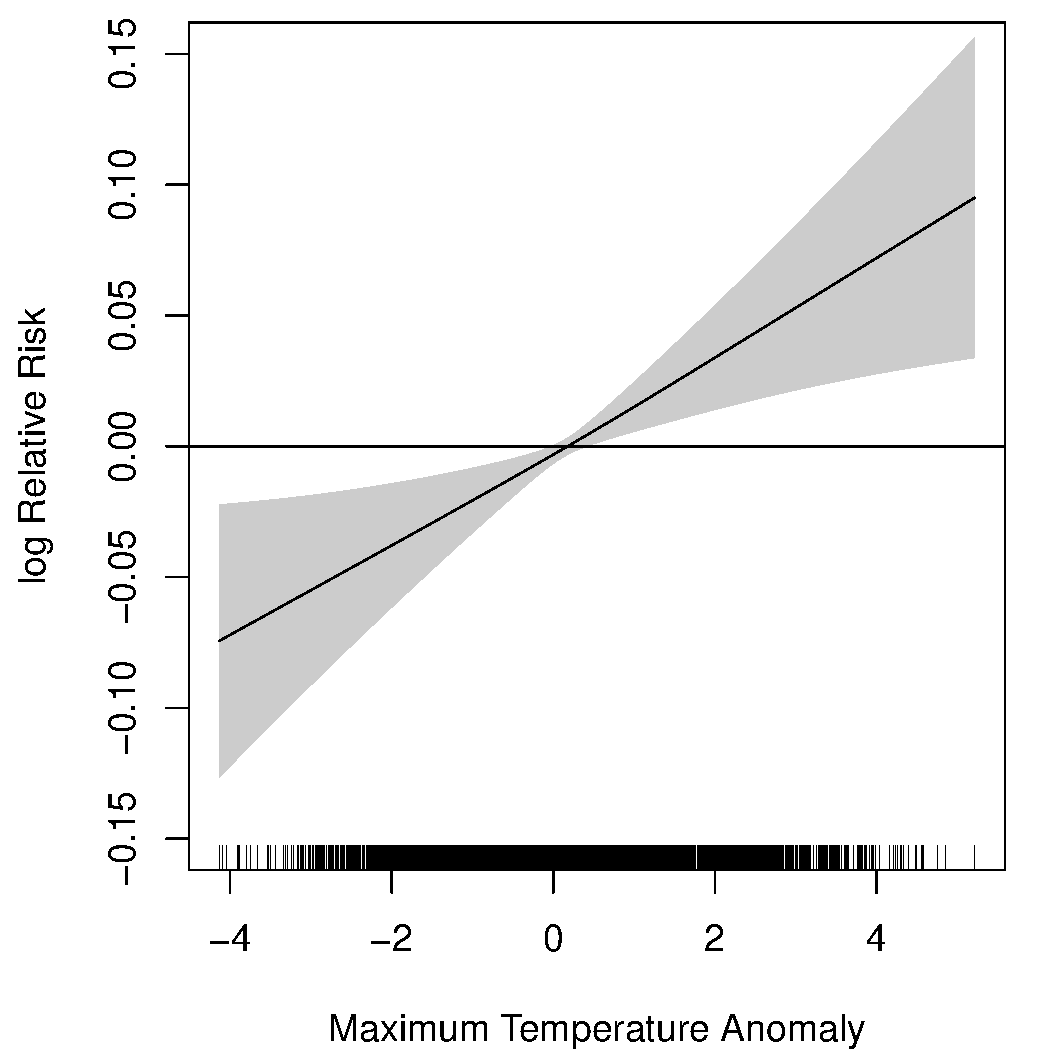
\includegraphics[width=.6\textwidth]{tmaxanom2.pdf}
\caption{2. Suicide/Temperature}
\label{fig:suigam}
\end{figure}
\end{block}

\begin{block}{Conclusions}
\begin{scriptsize}
This system:
\begin{itemize}
\item Enables data analysis in a safe environment
\item Allows comparison of multiple climate scenarios and assumptions
\item Demonstrated with a Climate/Health Impact Assessment
\end{itemize}
\begin{itemize}
\begin{large}
\item And this is Reproducible
\end{large}
\end{itemize}
\end{scriptsize}
\end{block}
\end{textblock}

\begin{textblock}{17}(40.5,47)

\begin{block}{References}
\begin{tiny}
\begin{thebibliography}{1}

\bibitem{Peng2011}
Roger~D. Peng.
\newblock {Reproducible research in computational science.}
\newblock {\em Science}, 334(6060), December 2011.

\bibitem{King1995}
Gary King.
\newblock {Replication, replication}.
\newblock {\em Political Science and Politics}, 28(3), September 1995.

\bibitem{Hanigan2012b}
Ivan~C. Hanigan, Colin~D. Butler, Phillip~N. Kokic, and Michael~F.~Hutchinson.
\newblock {Suicide and drought in New South Wales, Australia, 1970-2007}.
\newblock {\em Proceedings of the National Academy of Sciences}, 109(35), August~2012.

\bibitem{Climate2008}
Hilary~J. Bambrick, Keith~B.G. Dear, Rosalie~E. Woodruff, Ivan~C.~Hanigan, and
  Anthony~J. McMichael.
\newblock {The impacts of climate change on three health outcomes:
  temperature-related mortality and hospitalisations, salmonellosis and other
  bacterial gastroenteritis, and population at risk from dengue.}
\newblock Technical report, Garnaut Climate Change Review, Canberra, 2008.

\end{thebibliography}
\end{tiny}
\end{block}

\begin{block}{Acknowledgements}    
\begin{tiny}
\begin{itemize}
\item $^1$National Centre for Epidemiology and Population Health, ANU
\item $^2$Information Technology Services, ANU
\item $^3$Australian Data Archive, ANU 
\end{itemize}

\includegraphics[width=7cm]{ANU_LOGO_cmyk_56mm.png}

\includegraphics[width=4cm]{andslogo.pdf}

\includegraphics[width=6cm]{deptlogo.pdf} \\
This project is supported by the Australian National Data Service through the National Collaborative Research Infrastructure Strategy Program and the Education Investment Fund (EIF) Super Science Initiative.
\end{tiny}
\end{block}

\end{textblock}

\end{frame}
\end{document}
